\subsection{Vinkelberegning}

For at teste, om omregningen fra spændingen fra accelerometeret til grader fungerer i praksis, bevæges vinkeltesteren, der er vist på \autoref{fig:vinkeltest}, fra $180^{\circ}$ til $70^{\circ}$. Figur \ref{fig:spaending_vinkel_test} illustrer dette i MATLAB, hvor vinklen er illustreret på den venstre Y-akse, og hvor accelerometrenes spænding er illustreret på den højre Y-akse.

\begin{figure}[H]
\centering
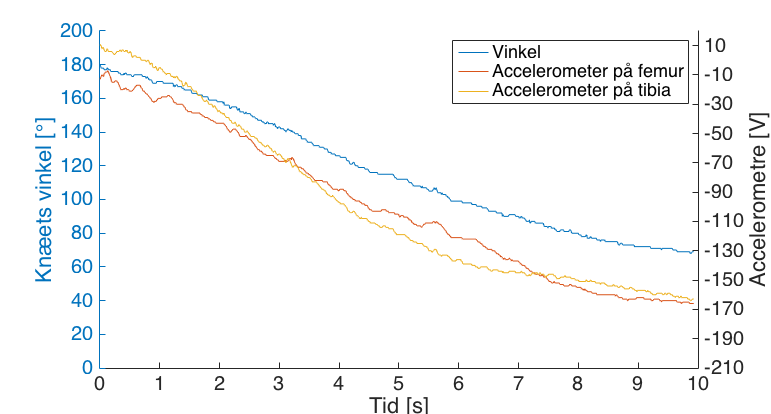
\includegraphics[width=1\textwidth]{figures/spaending_vinkel_test}
\caption{Test af vinkelberegning. Vinkel, som er den blå graf, er svarende til den samlede vinkel mellem de to accelerometre, hvor værdierne er illustreret på Y-aksen til venstre i grader. Spændingen målt for de to accelerometre måles i forhold til Y-aksen til højre og er vist ved en rød og gul graf.}
\label{fig:spaending_vinkel_test}
\end{figure}

\noindent
Det ses på \autoref{fig:spaending_vinkel_test}, at der er en sammenhæng mellem spænding og den samlede vinkel for accelerometrene. Der tages udgangspunkt i \autoref{tab:vinkelinterval_psoc} for omregningen, hvor spændingen for hvert accelerometer omregnes til grader. Disse lægges sammen for at udregne den samlede vinkel. Derudover illustrerer figuren, at vinklerne virker inden for det forventede arbejdsområde på $180^{\circ}$ til $90^{\circ}$, men ligeledes kan måle vinkler, der er lavere end $90^{\circ}$.

På figuren aflæses, at systemet registrerer en vinkel på $90^{\circ}$, når  accelerometeret på femur giver en spænding på $-0,2191~V$ og accelerometeret på tibia giver en spænding på $-0,2336~V$. 

For at teste, hvorvidt LED'en på mikrokontrolleren signalerer en vinkel under $90$ eller over $180^{\circ}$, indstilles vinkeltesten, hvilket ses af \autoref{fig:vinkeltest} brugt i pilotforsøget til henholdsvis $40^{\circ}$, $100^{\circ}$ og $200^{\circ}$. Hertil ses LED'en lyse grøn ved de acceptable grader mellem $90-180^{\circ}$, og rød ved grader udenfor graderne $90-180^{\circ}$. Dette ses af \autoref{fig:mikro_LED}.

\begin{figure}[H]
\centering
\includegraphics[width=1\textwidth]{figures/mikro_LED}
\caption{Mikrokontrollerens LED ses lyse grøn ved $100^{\circ}$ og lyse rød ved vinkler udenfor $90-180^{\circ}$.}
\label{fig:mikro_LED}
\end{figure}

Ved en overskridelse af grænsen for vinklen, skal det ligeledes visualiseres. Der er foretaget en test, hvorved acceleromterne er påsat en forsøgsperson som overstrækker i knæledder, hvorefter en squat udføres. En visualisering heraf ses af \autoref{fig:vinkeltest_graenser}.

\begin{figure}[H]
\centering
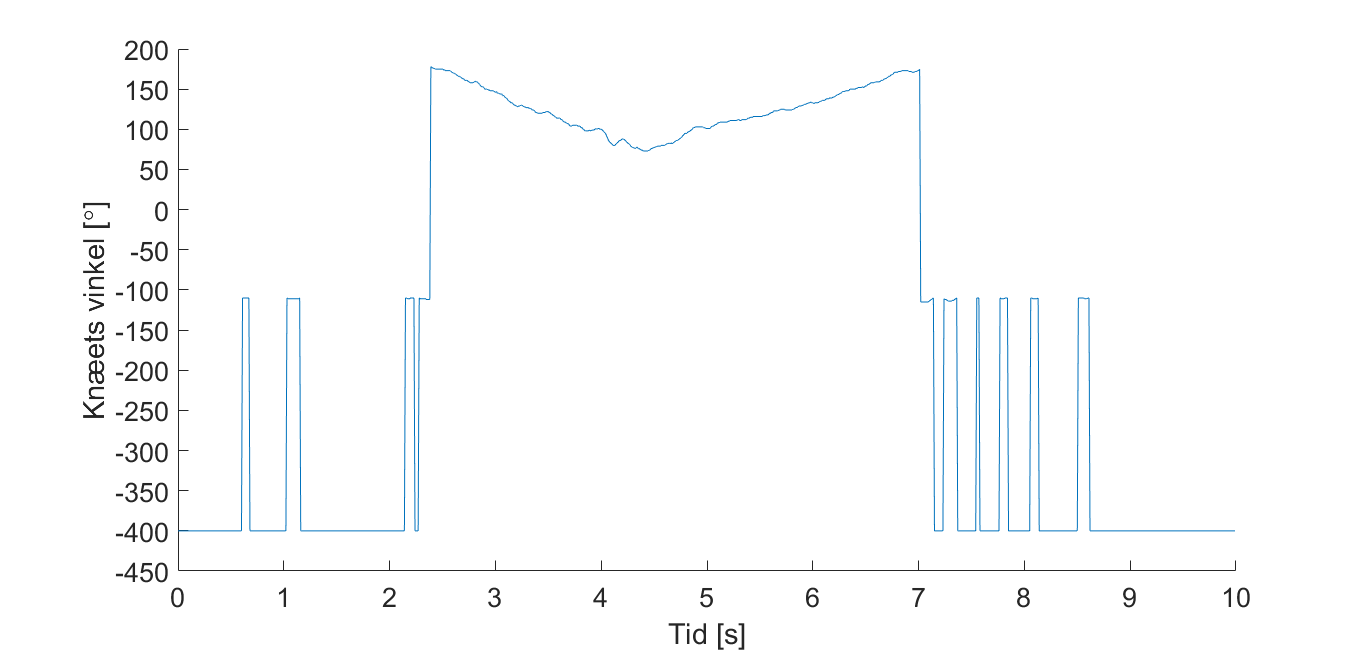
\includegraphics[width=1\textwidth]{figures/vinkeltest_graenser}
\caption{Grafen illustrerer vinklen over knæet under en squat-øvelse. Ved en vinkel under $-100^{\circ}$ symboliseres en overskridelse af grænsen for vinklen. }
\label{fig:vinkeltest_graenser}
\end{figure}

Det ses af \autoref{fig:vinkeltest_graenser}, at forsøgspersonen overstrækker knæleddet, således begge accelerometre overstiger grænsen på $90^{\circ}$, der til sammen udgør en samlet vinkel på $180^{\circ}$. Dette visualiseres ved en vinkel på $-400^{\circ}$. 
Efter 0,5 sekunder ses en vinkel på $-110^{\circ}$, hvilket er gældende, da det ene accelerometer har haft en spænding svarende til præcis $90^{\circ}$ og derfor ikke overskredet grænsen derpå. Ved squat-øvelsen begyndelse ses vinklen falde fra $180-73^{\circ}$, hvorefter den ses stigende igen. Til slut af målingen ses igen et fald under $-100^{\circ}$.



%Disse spændinger kan omregnes til vinkler ved først at finde, hvad spændingen er for én grad ud fra \autoref{tab:vinkelinterval_psoc}  i dét spændingsinterval, hvori den aflæste spænding befinder sig. Det kan aflæses i tabellen, at spændingen fra accelerometeret på femur giver en vinkel mellem 30 og $50^{\circ}$.
%
%\begin{equation}
%\dfrac{-143~V-(-84~V)}{20^{\circ}}=-2,95~V
%\end{equation}
%Derefter findes vinklen for accelerometeret.
%
%\begin{equation}
%\dfrac{-84~V+136~V}{2,95~V}+30^{\circ}=47,627^{\circ}
%\end{equation}
%Ligeledes kan vinklen fra accelerometeret på tibia udregnes til $41,429^{\circ}$. Dette giver en samlet vinkel over leddet: 
%%
%\begin{equation}
%47,627^{\circ}+41,429^{\circ}=89,056^{\circ}
%\end{equation}
%Dette giver en afvigelse på $-1,049~\%$ fra $90^{\circ}$. Denne afvigelse kan godtages til dette systems formål, da der ikke er nogen fare forbundet med, at systemet overskrider de opstillede grænser for vinkler med $-1,049~\%$.

\noindent
En yderligere test er foretaget for at undersøge forsinkelsen af vinkelberegning. Denne test er udført ved at definere en debug-pin, hvor pinen ved funktionskaldet sættes høj og lav efterfølgende. For at illustrere disse målinger tilsluttes et oscilloskop pinen, hvorved der måles hvornår denne er høj. Resultatet af denne test gav en forsinkelse på  $3.6~\mu~s$. Dette betragtes ikke som værende af signifikant betydning, hvorfor denne forsinkelse accepteres.


\vspace{3mm}
\textbf{Opsummering af krav:}
\begin{itemize}
\item[\text{\sffamily \checkmark}] Skal kunne udsende ét signal som repræsenterer en given vinkel
\item[\text{\sffamily \checkmark}] Skal kunne måle knæets vinkel mellem $180^{\circ}$ og $90^{\circ}$
\begin{itemize}
\item En grøn LED skal lyse, når knæets vinkel befinder sig inden for dette interval
\end{itemize}
\item[\text{\sffamily \checkmark}] Skal indikere, hvornår knæets vinkel er over $180^{\circ}$ og under $90^{\circ}$
\begin{itemize}
\item En rød LED skal lyse, hvis knæets vinkel er over $180^{\circ}$ eller under $90^{\circ}$
\end{itemize}
\item[\text{\sffamily \checkmark}] Skal indikere, hvornår knæet overstrækkes, hvilket svarer til $180^{\circ}$
\begin{itemize}
\item Hvis vinklen for ét accelerometer overstiger $90^{\circ}$, indikeres dette som $-200^{\circ}$, hvortil det andet accelerometers vinkel ligges til de $-200^{\circ}$
\item Hvis vinklen overstiger $90^{\circ}$ for hvert accelerometer, skal dette indikeres som et output på $-400^{\circ}$
\end{itemize}
\end{itemize}